%!TEX root = main.tex

Diseñe un código de Fano para una fuente con la siguiente distribución de probabilidad $$\{0.20, 0.19, 0.18, 0.17, 0.15, 0,10, 0.01\}$$.
\begin{sol}
    Este es el único ejercicio donde vamos a mostrar el proceso para crear un código de Fano, 
    primero organizamos las palabras de menor probabilidad a mayor y les asignamos un nombre
    $$
\begin{array}{|c|c|c|c|c|c|c|}
\hline
A & B & C & D & E & F & G\\
\hline
0.01& 0.10& 0.15& 0.17& 0.18& 0.19& 0.20\\
\hline

\end{array}
$$

    Y aplicamos el algoritmo, de la siguiente manera\\
    \begin{center}
     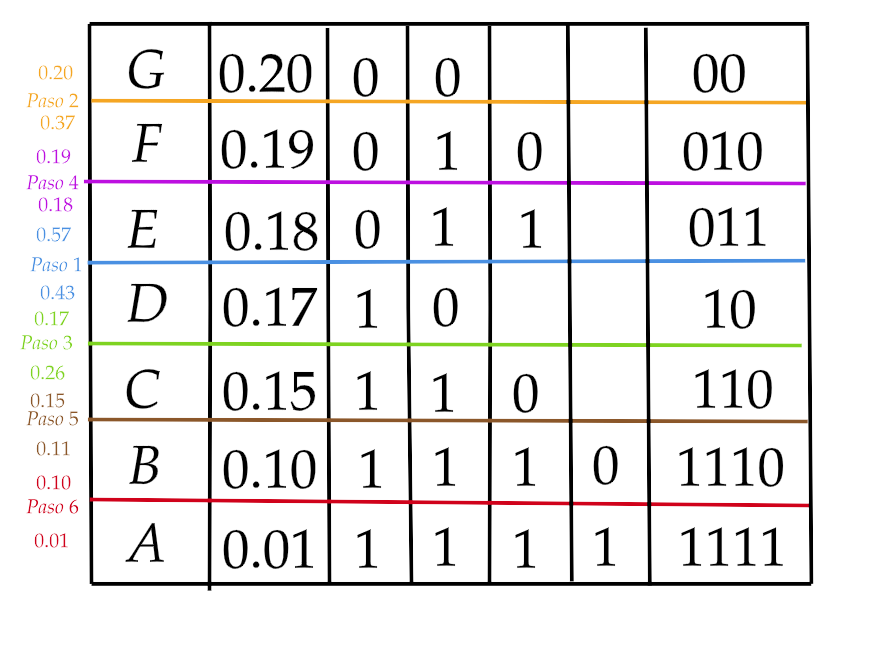
\includegraphics[scale=0.4]{diagrama.png}
    \end{center}
   
\end{sol}